\documentclass[twocolumn,prl,floatfix,superscriptaddress]{revtex4-2}
\usepackage{graphicx, subfigure, amsfonts, amssymb, amsmath, array, gensymb, fontenc, color, lipsum}
%\documentclass[aps,twocolumn,showpacs,preprintnumbers]{revtex4}
%\usepackage{graphicx}  % Include figure files
%\usepackage{subfigure}
%\usepackage{multirow}
%\linespread{1.0}
%\usepackage{fancyhdr}
%\usepackage{longtable}
%\usepackage{parskip}
%\usepackage[T1]{fontenc}
%\usepackage{dcolumn}
%\usepackage{bm}        
%\usepackage{amsfonts}  
%\usepackage{amsmath}   
%\usepackage{amssymb}
\usepackage{hyperref}
\usepackage{tikz}
\hypersetup{colorlinks= true, allcolors=blue}
%\setcitestyle{aysep={}}
%\setlength{\parindent}{11pt}
\frenchspacing

\newcommand\partitle[1]{\textsc{#1}.}
\begin{document}

\title{On the reality of the quantum state once again}
\author{Gabriele Carcassi}
\affiliation{Physics Department, University of Michigan, Ann Arbor, MI 48109}
\author{Andrea Oldofredi}
\affiliation{Centre of Philosophy, University of Lisbon, Portugal}
\author{Christine A. Aidala}
\affiliation{Physics Department, University of Michigan, Ann Arbor, MI 48109}
\vspace{2mm}

\date{\today}


\begin{abstract}
The Pusey, Barrett and Rudolph (PBR) theorem claims that quantum states cannot be taken to represent mere information about the system. This result is based on the ontological model framework proposed by Harrigan and Spekkens (HS). In this paper we show that the HS framework has a fundamental problem: the epistemic structure it implicitly assumes does not follow the one dictated by quantum mechanics. Namely, the map between the epistemic states of the model and quantum density matrices preserves neither the value nor ordering of the information entropy. Consequently the epistemic content of mixed states is not mapped in a meaningful way. The problem stems from the assumption that an epistemic state is characterized by a \emph{single} probability measure, which is essentially an assumption of non-contextuality. Given this fundamental issue, every result that uses the HS framework, including the PBR theorem, should be carefully reexamined.
\end{abstract}

\maketitle

\section{Introduction}
 
In 2012 Pusey, Barrett and Rudolph published a formal result in \emph{Nature Physics}, widely known as the PBR theorem, showing that ``if the quantum state merely represents information about the real physical state of a system, then experimental predictions are obtained that contradict those of quantum theory'' (\cite{PBR:2012}, p.\ 475). Alternatively stated, PBR argued that in every model reproducing the statistics and predictions of Quantum Mechanics (QM) the quantum state $\psi$ must represent real physical properties of the system under consideration and not agents' knowledge---i.e.\ models must be $\psi$-ontic. Consequently, quantum theories cannot be $\psi$-epistemic. 

Such a theorem had a remarkable resonance (\cite{Leifer:2014, Leifer:2014b, Renner:2012, Colbeck:2017, Hardy:2013, Maroney:2014, Patra:2013, Mansfield:2016, Schlosshauer:2012, Schlosshauer:2013, Schlosshauer:2014, Aaronson:2013}), and questions about its actual meaning are still discussed today: on the one hand, it rules out interpretations of QM where $\psi$ merely represents information. On the other, scholars recently showed that non-trivial epistemic as well as statistical approaches to QM are not refuted by the PBR argument (\cite{Ben:2017, Rizzi:2018, Oldofredi:2021, DeBrota:2019}).
	
In this paper we are not going to rebut the theorem itself. We instead aim to carefully reexamine one of its premises, i.e.\ Harrigan and Spekkens' (HS) classification between $\psi$-ontic and $\psi$-epistemic ontological models  \cite{Harrigan:2010} on top of which the PBR result is derived. We believe that a careful examination of this assumption forces us to reevaluate the significance of the PBR conclusion. 
		
HS proposed a rigorous classification in order to categorize the nature of the quantum state, i.e.\ to establish whether in a certain model $\psi$ corresponds to a real property of a quantum object, in which case the model is called $\psi$-ontic, or to some observer information, making it $\psi$-epistemic. While the original aim of this classification was to clarify Einstein's view of quantum theory, the HS framework has been widely employed in the literature not only to categorize different interpretations, but also to argue what types of interpretations are admissible (\cite{Leifer:2013, Leifer:2017, Branciard:2014, Hermens:2021, Wood:2015, Ringbauer:2015, Mazurek:2016, Bartlett:2012}; cf.\ \cite{Oldofredi:2020b, Lewis:2012, Ladyman:2021} for critical discussions). Given the influence that the HS framework and the PBR theorem have in quantum foundations, it is worthwhile to look again at the former with more scrutiny in order to understand whether it is a sound basis from which to draw conclusions on the nature of the quantum state.

In this paper we will show two things:
\begin{enumerate}
	\item the information entropy as calculated on HS epistemic states does not match the one provided by quantum mechanics, therefore the epistemic structures provided by QM and HS are not isomorphic;
	\item if we rephrase the overlapping condition directly in terms of density matrices, we find that non-orthogonal pure states ``overlap'', which rules out $\psi$-ontic models.
\end{enumerate}
Combining these results with PBR, our conclusion is that the HS classification itself is fundamentally problematic. The main issue lies in assuming that the epistemic state identifies a \emph{single} probability distribution over the whole set of ontic states. We show that this, in essence, is an assumption of non-contextuality, which is also inherited by the PBR theorem, casting doubts on its validity.

\section{Summary of the Harrigan \& Spekkens Model}

We briefly review the main features of the classification provided by HS starting with the usual operational setting for QM. We have a preparation protocol $P$, associated with a density operator $\rho$ on the relevant Hilbert space, and a measurement protocol $M$, represented by a POVM $\{ E_k\}$ where each $k$ represents a possible measurement outcome. The probability of obtaining a particular $k$ given a particular preparation $P$ and measurement $M$ is given by the generalized Born rule
\begin{equation}
	p(k|M, P)=\textrm{tr}(\rho E_k).
\end{equation}

An ontological model, as defined by HS, additionally assumes that there exists a set of states $\Lambda$, called \textbf{ontic states}, that provide the complete specification of the properties of a given physical object. A preparation $P$ will prepare a particular ontic state $\lambda$ according to the probability distribution $p(\lambda | P)$, which is referred to as \textbf{epistemic state}. The measurement outcome will depend only on the ontic state with probability $p(k|\lambda, M)$ (\cite{Harrigan:2010}, p.\ 128). This leads to the following expression:
\begin{equation}
	\int_\Lambda d\lambda p(k|\lambda, M) p(\lambda| P)= \textrm{tr}(\rho E_k).
\end{equation}
It is also assumed that a mixture of pure states $\{ \psi_i \}$ with probabilities $\{ w_i \}$ will be represented by
\begin{equation}\label{epistemic_mixing}
	\sum_i  w_i p(\lambda| P_{\psi_i}).
\end{equation}
As the epistemic states for mixed preparations are simply linear combinations of epistemic states for pure preparations, the HS model concentrates on the latter.

To classify an ontological model, we look at the relationship between quantum and ontic states. There are two broad categories. In a \textbf{$\psi$-ontic} model the wave function is a physical property of the ontic state, in the sense that given an ontic state $\lambda$ there is only one pure state preparation $P_\psi$ that could have prepared $\lambda$. As we can see in figure \ref{overlap}, this happens if the probability distributions do not overlap, i.e.\ if we have
\begin{equation}\label{ontic_condition}
	p(\lambda | P_{\psi})p(\lambda|P_{\phi})=0
\end{equation}
for all pairs of states $\psi$ and $\phi$. If a model is not $\psi$-ontic, then it is \textbf{$\psi$-epistemic}. In this case, $\lambda$ can be described by more than one quantum state and the wave function is taken to represent knowledge about the state preparation---in such models quantum states generate overlapping probability distributions over $\Lambda$ as shown in figure \ref{overlap} (b). A $\psi$-ontic model is said \textbf{$\psi$-complete} if the quantum states and the ontic states coincide. More precisely if 
\begin{equation}\label{complete_condition}
	p(\lambda|P_\psi)=\delta(\lambda-\lambda_{\psi}).
\end{equation}
All other models are \textbf{$\psi$-incomplete}.

To make this classification more concrete, let us give an example from classical mechanics. Consider the case where we prepare a particle according to a specific value of energy. The energy partitions phase space into mutually exclusive regions, and therefore we can understand the energy of the preparation as a property of the particle itself. According to HS, this would be an \emph{ontic property}. Consider now the case where we prepare a particle according to a specific temperature. When we take the particle from the oven, we are sampling from a Boltzmann distribution over different energies. However, unlike energy, temperature does not partition phase space because the same particle state could have been prepared by ovens at different temperature. Temperature is a property of the preparation and therefore an \emph{epistemic property}. 

\begin{figure}
\includegraphics[scale=.7]{ontic}
\caption{\footnotesize{Harrigan and Spekkens' distinction between $\psi$-ontic (a) and $\psi$-epistemic (b) ontological models.}}\label{overlap}
\end{figure}


\section{Entropy and the ontological model}

To reproduce quantum theory, an ontological model has to reproduce not simply the probability of transitions during measurements but also all the results of quantum statistical mechanics and quantum information theory. Therefore it has to reproduce the correct values for entropy of mixed states. The natural way is by using standard information theoretic tools over the space of epistemic states which, as we will see, rules out $\psi$-ontic models. The degree of overlap between distributions, in fact, is not a choice, but is fixed by the value of entropy.

Let us first review a crucial property of the information entropy, both in the classical setting (i.e.\ the Shannon/Gibbs entropy) and in the quantum setting (i.e.\ the von Neumann entropy).\footnote{We show the explicit calculations in the appendix.}

\textbf{Classical information entropy of mixed non-overlapping distributions}. Let $\rho_1$ and $\rho_2$ be two classical distributions over a space $\Lambda$ with measure $\lambda$. The entropy for each distribution is given by the usual formula\footnote{The logarithm is assumed to be in base 2.}, for example
\begin{equation}\label{shannon_entropy}
	H(\rho_1) = - \int_\Lambda \rho_1(\lambda) \log \rho_1(\lambda) d\lambda.
\end{equation}
Suppose the two distributions are disjoint, and let $\rho = \frac{1}{2} \rho_1 + \frac{1}{2} \rho_2$ be a uniform mixture of the two distributions. The entropy of $\rho$ is given by
\begin{equation}\label{entropy_nonoverlap}
	H(\rho) = 1 + \frac{1}{2} H(\rho_1) + \frac{1}{2} H(\rho_2).
\end{equation}
Note how the non-overlapping assumption fixes the entropy of the mixed state.

\textbf{Quantum information entropy of quantum mixed states}. Now suppose $\psi$ and $\phi$ are two pure quantum states and let $p = | \langle \psi | \phi \rangle |^2$ be the probability of transition from one to the other. Consider the mixed state $\rho = \frac{1}{2} | \psi \rangle \langle \psi | + \frac{1}{2} | \phi \rangle \langle \phi |$. Its entropy is given by
\begin{equation}\label{entropy_mixed}
	H(\rho) = H\left(\frac{1+\sqrt{p}}{2}, \frac{1-\sqrt{p}}{2}\right).
\end{equation}

\emph{\textbf{Theorem: Since non-overlapping distributions can only represent orthogonal states, $\psi$-ontic models cannot be consistent with quantum theory.}}

\emph{Proof}: Suppose we have a $\psi$-ontic model defined according to \cite{Harrigan:2010}. The epistemic states $p(\lambda|P_\psi)$ and $p(\lambda|P_\phi)$ consist of non-overlapping distributions over a space $\Lambda$, therefore eq. \ref{entropy_nonoverlap} applies. Given that $\psi$ and $\phi$ are pure states, and the entropy for pure states is zero, we must have
\begin{equation}\label{entropy_pure}
	H(p(\lambda|P_\psi)) = H(p(\lambda|P_\phi)) = 0,
\end{equation}
and therefore
\begin{equation}\label{required_entropy}
	\begin{aligned}
		H\left(p(\lambda|\frac{1}{2}P_\psi + \frac{1}{2}P_\phi)\right) &= \\
		H\left(\frac{1}{2}p(\lambda|P_\psi) + \frac{1}{2}p(\lambda|P_\phi)\right) 
		&= 1.
	\end{aligned}
\end{equation}
If we compare the above with eq.~\ref{entropy_mixed}, it follows that $p$ must be zero. That is, we must have that
\begin{equation}\label{orthogonal}
	\langle \psi | \phi \rangle = 0
\end{equation}
no matter what $\psi$ and $\phi$ are.

Hence, the non-overlapping assumption built into the $\psi$-ontic model necessarily implies that all pure states are orthogonal. Since this is not true in quantum mechanics, any $\psi$-ontic model will fail to reproduce the results of quantum information, quantum statistical mechanics and, therefore, quantum theory in general. $\square$

We should also note that one has problems for $\psi$-epistemic models. While PBR leaves the possibility of $\psi$-epistemic models that use correlations, the correlations is also fixed by the entropy. It is a well-known result  [CITE: libri di informazione] in both classical and quantum information theory that the entropy of a joint distribution of the marginal if and only if the subsystems are independent. Therefore an epistemic state that represents independent quantum states must also be the joint distribution of statistically independent epistemic states of the individual systems. This, combined with PBR, tells us that no models can reproduce quantum statistical mechanics and quantum information theory.

The conclusion is the following:
\begin{quote}
	\textbf{no ontological model can reproduce quantum statistical mechanics and quantum information with standard information theoretic tools}.
\end{quote}
That is, even if one had an ontological model that mapped the result of single outcome correctly, it would still give the wrong answer when trying to calculate ensembles and their entropy.

In principle, we do not exclude that someone may find a different construction to reproduce the correct entropies. There are, however, at least two objective difficulties that cannot be circumvented. First of all, information entropy is strictly concave, meaning that $H(p \rho_1 + (1-p) \rho_2) \geq p H(\rho_1) + (1-p) H(\rho_2)$ with the equality valid only if $\rho_1$ and $\rho_2$ are the same exact state. Therefore entropy fixed equality. Because the mapping between epistemic states and density matrices is not injective,\footnote{Quantum mixture do not have a single decomposition in pure states. For example, the maximally mixed state of a qubit can be achieved with either an equal mixture of spin up and down or an equal mixture of spin left and right.} epistemic states must form equivalence classes and the strict concavity must be lost. That is, one can make mixtures of different ensemble without increasing entropy.

Secondly, as equation \ref{entropy_mixed} shows, the compute of the entropy requires the inner product. Therefore, whatever other structure one puts on top of epistemic states, essentially redefines the inner product. In other words, the idea that the inner product just represent transition probabilities, which, in our view, is the key idea the ontological model uses to explain ``what really happens'' does not work.

Furthermore, we stress that it is not our place to solve these problems: we are not the proponent of this model. Our only aim is to raise enough doubt that the ontological model, as it currently stand, is highly problematic.

\section{Conclusion}

We showed not only that the HS framework does not correctly describe the epistemic structure of QM, but also that it implicitly assumes non-contextuality. Hence, it cannot be employed to draw conclusions on the nature of quantum states. Consequently, any other result relying on the HS categorization inherits the same issues. In particular, it follows that the PBR theorem is derived from a technically ill-defined basis; thus, it is demonstrated neither that quantum states must necessarily be HS-$\psi$-ontic, nor that epistemic interpretations are contradicted by quantum theory. Concluding, we believe that while work in quantum foundations typically focuses on measurements and their effect on pure states, equal importance must be given to preparations and their effect on mixed states. The different behavior of entropy in classical and quantum mechanics has profound implications not just for information theory, but also for statistical mechanics and its measurable predictions. 

%A full solution to the ``measurement problem'' will therefore have to address the dual ``preparation problem.''

%Number of words for the conclusion: 164

\section{Acknowledgements}

Andrea Oldofredi is grateful to the Funda\c{c}$\tilde{\mathrm{a}}$o para a Ci\^encia e a Tecnologia (FCT) for financial support (Grant no. 2020.02858.CEECIND).  This work is in connection to Assumptions of Physics, a larger project that aims to identify a handful of physical principles from which the basic laws can be rigorously derived  (\url{https://assumptionsofphysics.org}).

%\bibliographystyle{ieeetr}
\bibliography{bibliography}
\clearpage

\section*{Appendix: calculation}
\label{A}
\textbf{Entropy of mixed non-overlapping distributions}. We want to show that, given two non-overlapping probability distributions $\rho_1$ and $\rho_2$, the entropy of $\rho = \frac{1}{2} \rho_1 + \frac{1}{2} \rho_2$ is given by
\begin{equation}
	H(\rho) = 1 + \frac{1}{2} H(\rho_1) + \frac{1}{2} H(\rho_2). \tag{\ref{entropy_nonoverlap}}
\end{equation}

Let $U_1, U_2 \subset \Lambda$ be the respective supports of the distributions. Since the distributions are non-overlapping, we have $U_1 \cap U_2 = \emptyset$. We have
\begin{align*}
	H(\rho) &= - \int_\Lambda \rho \log \rho d\lambda \\
	&= -\int_{U_1} \rho \log \rho d\lambda -\int_{U_2} \rho \log \rho d\lambda \\
	&= -\int_{U_1} \frac{1}{2} \rho_1 \log \frac{1}{2} \rho_1 d\lambda -\int_{U_2} \frac{1}{2} \rho_2 \log \frac{1}{2} \rho_2 d\lambda \\
	&= - \frac{1}{2} \int_{U_1} \rho_1 \log \frac{1}{2} d\lambda - \frac{1}{2} \int_{U_1} \rho_1 \log \rho_1 d\lambda \\
	&- \frac{1}{2} \int_{U_2} \rho_2 \log \frac{1}{2} d\lambda - \frac{1}{2} \int_{U_2} \rho_2 \log \rho_2 d\lambda \\
	&= - \frac{1}{2} \log \frac{1}{2} - \frac{1}{2} \log \frac{1}{2} + \frac{1}{2} H(\rho_1) + \frac{1}{2} H(\rho_2) \\
	&= 1 + \frac{1}{2} H(\rho_1) + \frac{1}{2} H(\rho_2). \\
\end{align*}


\textbf{Entropy of quantum mixed states}. We want to show that, given two states $\psi$ and $\phi$, the entropy of the mixed state $\rho = \frac{1}{2}|\psi\rangle\langle\psi| + \frac{1}{2}|\phi\rangle\langle\phi|$ is
\begin{equation}\label{entropy}
	H(\rho) = H\left(\frac{1+|\langle\psi|\phi\rangle|}{2}, \frac{1-|\langle\psi|\phi\rangle|}{2}\right).
\end{equation}

\begin{center}
	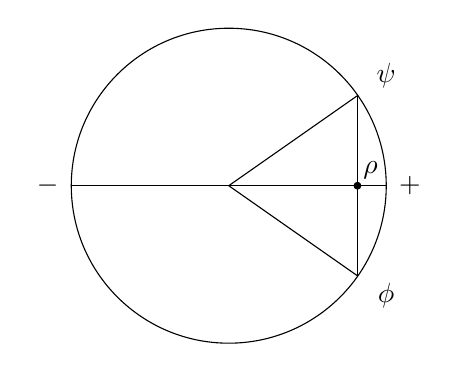
\begin{tikzpicture}[scale = 1]
		\draw (0,0) circle (2);
		\node at (-2.3,0) {$-$};
		\node at (2.3,0) {$+$};
		\node at (2,1.4) {$\psi$};
		\node at (2,-1.4) {$\phi$};
		\draw (-2,0) -- (2,0);
		\begin{scope}
			\clip(0,0) circle (2);
			\draw (0,0) -- (2,1.4);
			\draw (0,0) -- (2,-1.4);
			\draw (1.634,1.4) -- (1.634,-1.4);
		\end{scope}
		\fill (1.634,0) circle (0.05);
		\node at (1.8,.2) {$\rho$};
	\end{tikzpicture}
\end{center}

Note that $\psi$ and $\phi$ will identify a two-dimensional subspace which can be thought, without loss of generality, as a qubit and therefore can be represented by a Bloch sphere. The picture represents the intersection of the Bloch sphere with the plane identified by $\psi$ and $\phi$. As $\rho$ is an equal mixture of the two states, it will be represent by the midpoint between the two. Taking the line that goes through $\rho$ and the center of the sphere, we can see that $\rho$ can also be seen as the mixture of the states $+$ and $-$ which, since they represent equal and opposite directions, form a basis. To diagonalize $\rho$, then, means to express it in terms of $+$ and $-$.

If $\theta_{\psi\phi}$ is the angle between $\psi$ and $\phi$, we have
\begin{equation}
	|\langle \psi | \phi \rangle |^2 = \cos^2 \frac{\theta_{\psi\phi}}{2}.
\end{equation}
The angle is divided by two because the angle on the Bloch sphere (i.e. in physical space) is double the angle in the Hilbert space. For example, for $z^+$ and $z^-$ the angle on the Bloch sphere would be $\pi$ and the inner product is zero (i.e. opposite directions in physical space correspond to orthogonal states).

Now we express $\psi$ and $\phi$ in terms of $+$ and $-$, remembering that they form a basis. Given that $\rho$ is at the midpoint, the figure is vertically symmetric. The angle between $\psi$ and $+$, then, is half of $\theta_{\psi\phi}$. The inner product between $\psi$ and $+$ is
\begin{equation}
	\begin{aligned}
		|\langle \psi | + \rangle |^2 &= \cos^2 \frac{\theta_{\psi +}}{2} \\
		&= \cos^2 \frac{\theta_{\psi\phi}}{4}.
	\end{aligned}
\end{equation}
Keeping in mind that we are composing vectors in the Hilbert space (and not in the geometry of the physical space) we have
\begin{align*}
	\left|\psi\right>&=\cos\frac{\theta_{\psi\phi}}{4}\left|+\right>+\sin\frac{\theta_{\psi\phi}}{4}\left|-\right> \\
	\left|\phi\right>&=\cos\frac{\theta_{\psi\phi}}{4}\left|+\right>-\sin\frac{\theta_{\psi\phi}}{4}\left|-\right>.
\end{align*}

The density matrices corresponding to the pure states are
\begin{align*}
	\left|\psi\right>\left<\psi\right|&=\cos^2\frac{\theta_{\psi\phi}}{4}\left|+\right>\left<+\right|\\
	&+\cos\frac{\theta_{\psi\phi}}{4}\sin\frac{\theta_{\psi\phi}}{4}\left(\left|+\right>\left<-\right|+\left|-\right>\left<+\right|\right) \\
	&+\sin^2\frac{\theta_{\psi\phi}}{4}\left|-\right>\left<-\right| \\
	\left|\phi\right>\left<\phi\right|&=\cos^2\frac{\theta_{\psi\phi}}{4}\left|+\right>\left<+\right|\\
	&-\cos\frac{\theta_{\psi\phi}}{4}\sin\frac{\theta_{\psi\phi}}{4}\left(\left|+\right>\left<-\right|+\left|-\right>\left<+\right|\right) \\
	&+\sin^2\frac{\theta_{\psi\phi}}{4}\left|-\right>\left<-\right|.
\end{align*}

We can now calculate the mixture
\begin{align*}
	\frac{1}{2}(|\psi\rangle\langle\psi| &+ |\phi\rangle\langle\phi|) \\
	&=\cos^2\frac{\theta_{\psi\phi}}{4}\left|+\right>\left<+\right| +\sin^2\frac{\theta_{\psi\phi}}{4}\left|-\right>\left<-\right| \\
	&=\frac{1+\cos\frac{\theta_{\psi\phi}}{2}}{2}\left|+\right>\left<+\right| +\frac{1-\cos\frac{\theta_{\psi\phi}}{2}}{2}\left|-\right>\left<-\right| \\
	&=\frac{1+|\langle\psi|\phi\rangle|}{2}\left|+\right>\left<+\right| +\frac{1-|\langle\psi|\phi\rangle|}{2}\left|-\right>\left<-\right|. \\
\end{align*}

As $\rho$ is in a diagonal form, the entropy is given by eq.~\ref{entropy}.


\end{document}